\chapter{Задание}


\begin{enumerate}
	\item Для выборки объема $n$ из нормальной генеральной совокупности $X$ реализовать в виде программы на ЭВМ
	\begin{enumerate}
		\item вычисление точечных оценок $\hat\mu(\vec x_n)$ и $S^2(\vec x_n)$ математического ожидания $MX$ и дисперсии $DX$ соответственно;
		\item вычисление нижней и верхней границ $\underline\mu(\vec x_n)$, $\overline\mu(\vec x_n)$ для $\gamma$-доверительного интервала для математического ожидания $MX$;
		\item вычисление нижней и верхней границ $\underline\sigma^2(\vec x_n)$, $\overline\sigma^2(\vec x_n)$ для $\gamma$-доверительного интервала для дисперсии $DX$;
	\end{enumerate}
	\item вычислить $\hat\mu$ и $S^2$ для выборки из индивидуального варианта;
	\item для заданного пользователем уровня доверия $\gamma$ и $N$ – объема выборки из индивидуального варианта:
	\begin{enumerate}
		\item на координатной плоскости $Oyn$ построить прямую $y = \hat\mu(\vec{x_N})$, также графики функций $y = \hat\mu(\vec x_n)$, $y = \underline\mu(\vec x_n)$ и $y = \overline\mu(\vec x_n)$ как функций объема $n$ выборки, где $n$ изменяется от 1 до $N$;
		\item на другой координатной плоскости $Ozn$ построить прямую $z = S^2(\vec{x_N})$, также графики функций $z = S^2(\vec x_n)$, $z = \underline\sigma^2(\vec x_n)$ и $z = \overline\sigma^2(\vec x_n)$ как функций объема $n$ выборки, где $n$ изменяется от 1 до $N$.
	\end{enumerate}
\end{enumerate}



%\textbf{Выборка индивидуального варианта №8:}

%\begin{lstlisting}
%X=(7.76,6.34,5.11,7.62,8.84,4.68,8.65,6.90,8.79,6.61,6.62,7.13,6.75,7.28,7.74,7.08,5.57,8.20,7.78,7.92,6.00,4.88,6.75,6.56,7.48,8.51,9.06,6.94,6.93,7.79,5.71,5.93,6.81,5.76,5.88,7.05,7.22,6.67,5.59,6.57,7.28,6.22,6.31,5.51,6.69,7.12,7.40,6.86,7.28,6.82,7.08,7.52,6.81,7.55,4.89,5.48,7.74,5.10,8.17,7.67,7.07,5.80,6.10,7.15,7.88,9.06,6.85,4.88,6.74,8.76,8.53,6.72,7.21,7.42,8.29,8.56,9.25,6.63,7.49,6.67,6.79,5.19,8.20,7.97,8.64,7.36,6.72,5.90,5.53,6.44,7.35,5.18,8.25,5.68,6.29,6.69,6.08,7.42,7.10,7.14,7.10,6.60,6.35,5.99,6.17,9.05,6.01,7.77,6.27,5.81,7.80,9.89,4.39,6.83,6.53,8.15,6.68,6.87,6.31,6.83)
%\end{lstlisting}

\chapter{Теоретические сведения}

\section{Определение $\gamma$-доверительного интервала для значения параметра распределения случайной величины}

Пусть X -- случайная величина, закон распределения которой известен с точностью до неизвестного параметра $\theta$. 

\textbf{Определение.}

Интервальной оценкой параметра $\theta$ уровня $\gamma$ ($\gamma$-интервальной оценкой) называют пару статистик $\underline{\theta}(\vec X) \text{ и } \overline{\theta}(\vec X)$ таких, что $$P\{\theta \in (\underline{\theta}(\vec X), \overline{\theta}(\vec X))\}=\gamma$$ 


\textbf{Определение.}
$\gamma$-доверительным интервалом (доверительным интервалом уровня $\gamma$) для параметра $\theta$ называют реализацию (выборочное значение) интервальной оценки уровня $\gamma$ для этого параметра, то есть интервал $(\underline{\theta}(\vec x), \overline{\theta}(\vec x))$ с детерминированными границами.


\section{Формулы для вычисления границ \\ $\gamma$-доверительного интервала для математического ожидания и дисперсии нормальной случайной величины.}

Формулы для вычисления границ $\gamma$-доверительного интервала для математического ожидания нормальной случайной величины:

$$
\underline\mu(\vec X_n)=\overline X - \frac{S(\vec X)t^{(n-1)}_{\frac{1+\gamma}{2}}}{\sqrt{n}},
$$

$$
\overline\mu(\vec X_n)=\overline X + \frac{S(\vec X)t^{(n-1)}_{\frac{1+\gamma}{2}}}{\sqrt{n}},
$$
где $\overline X$ -- выборочное среднее, $S^2(\vec X)$ -- исправленная выборочная дисперсия, $n$ -- объем выборки, $\gamma$ -- уровень доверия, $t^{(n-1)}_{\frac{1+\gamma}{2}}$ -- квантиль уровня $\frac{1+\gamma}{2}$ распределения Стьюдента с n-1 степенью свободы.

Формулы для вычисления границ $\gamma$-доверительного интервала для дисперсии нормальной случайной величины:

$$
\underline\sigma^2(\vec X_n)= \frac{(n-1)S^2(\vec X)}{h^{(n-1)}_{\frac{1+\gamma}{2}}},
$$

$$
\overline\sigma^2(\vec X_n)= \frac{(n-1)S^2(\vec X)}{h^{(n-1)}_{\frac{1-\gamma}{2}}},
$$
где $S^2(\vec X)$ -- исправленная выборочная дисперсия, $n$ -- объем выборки, $\gamma$ -- уровень доверия, $h^{(n-1)}_{\alpha}$ -- квантиль уровня $\alpha$ распределения $\chi^2$ с n - 1 степенью свободы.


\chapter{Результаты работы}

\section{Текст программы}


\lstinputlisting[style=mstyle]{../main_my.m}

\section{Результаты работы программы}


\begin{equation*}
	\hat\mu(\vec x_n) = 6.944500\\
\end{equation*}
\begin{equation*}
	S^2(\vec x_n) = 1.171956\\
\end{equation*}
\begin{equation*}
	\underline\mu(\vec x_n) = 6.780673\\
\end{equation*}
\begin{equation*}
	\overline\mu(\vec x_n) = 7.108327 \\
\end{equation*}
\begin{equation*}
	\underline{S^2}(\vec x_n) = 0.958766\\
\end{equation*}
\begin{equation*}
	\overline{S^2}(\vec x_n) = 1.470952\\
\end{equation*}



\newpage

\begin{figure}[ht!]	
	\centering{
		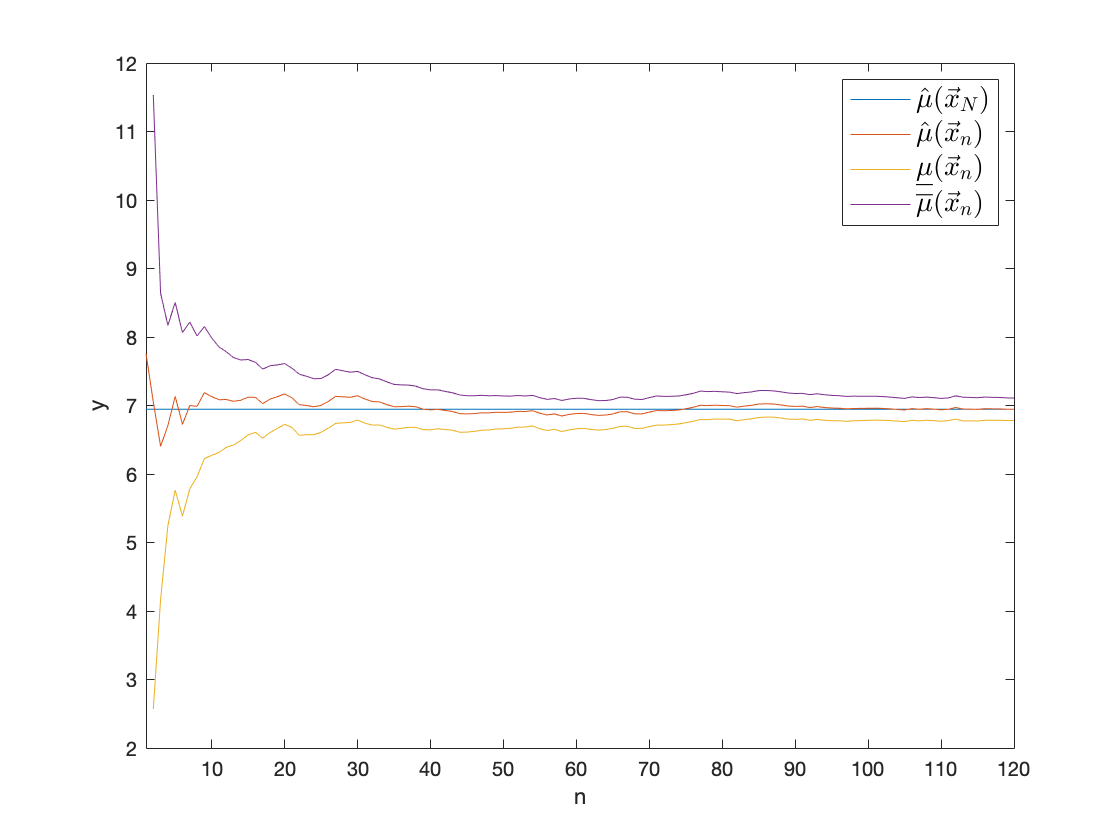
\includegraphics[scale=0.5]{p1.png}
		\caption{Прямая $y = \hat\mu(\vec x_N)$, а также графики функций  $y(n) = \hat\mu(\vec x_n)$, $y(n) = \underline\mu(\vec x_n)$, $y(n) = \overline\mu(\vec x_n)$ как функций объема $n$ выборки, где $n$ изменяется от 1 до $N$}}
\end{figure}


\begin{figure}[ht!]	
	\centering{
		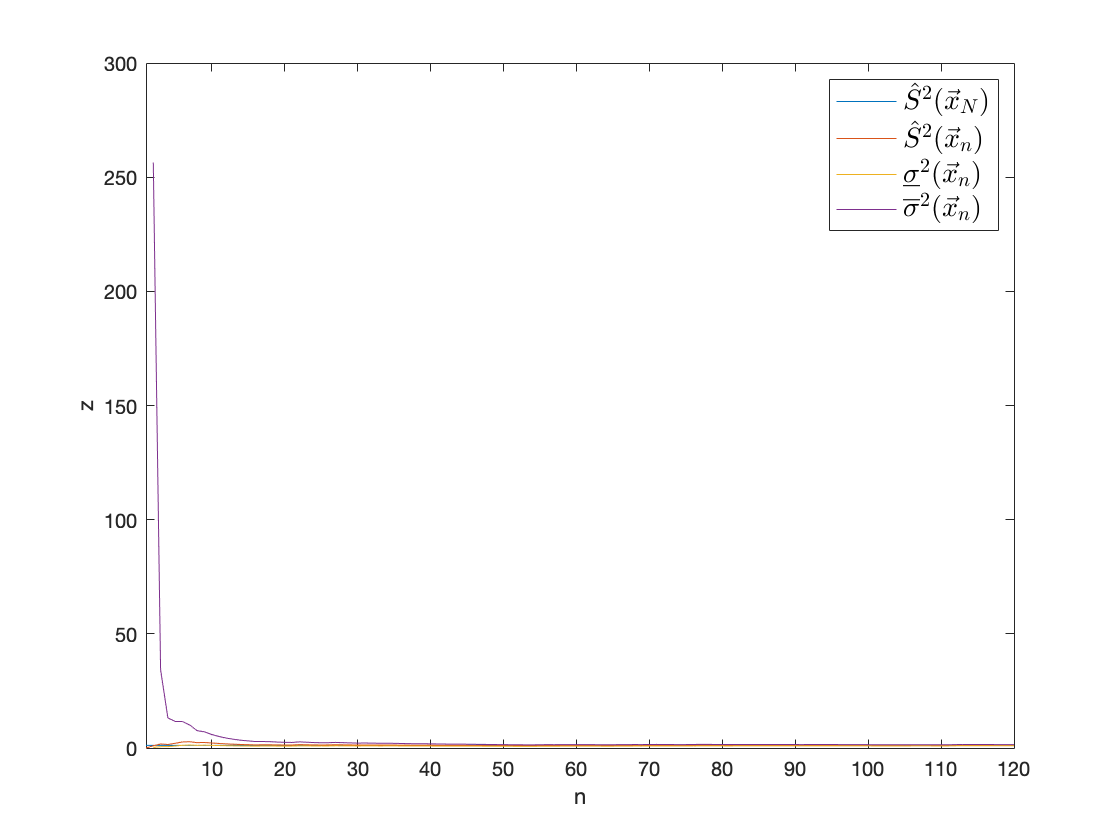
\includegraphics[scale=0.5]{p2.png}
		\caption{Прямая $z = S^2(\vec x_N)$, а также графики функций $z(n) = S^2(\vec x_n)$, $z(n) = \underline \sigma^2(\vec x_n)$, $z(n) = \overline \sigma^2(\vec x_n)$ как функций объема $n$ выборки, где $n$ изменяется от 1 до $N$}}
\end{figure}
